\documentclass{standalone}

\usepackage{tikz}

\begin{document}
  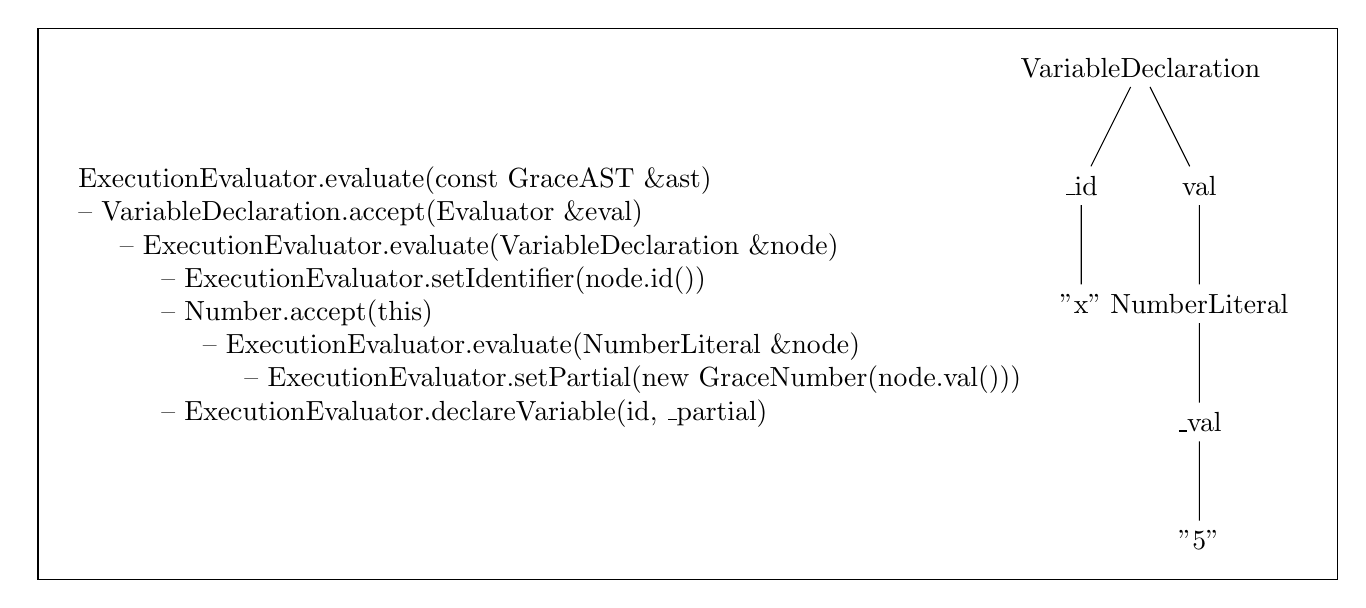
\begin{tikzpicture}
  	\node[align=left] at (0,-1) {
  	\parindent=3em  
  	 \\ \\
\indent ExecutionEvaluator.evaluate(const GraceAST \&ast)\\
\indent -- VariableDeclaration.accept(Evaluator \&eval)\\
 \indent\indent -- ExecutionEvaluator.evaluate(VariableDeclaration \&node)\\
 \indent\indent\indent -- ExecutionEvaluator.setIdentifier(node.id())\\ 
 \indent\indent\indent -- Number.accept(this)\\
 \indent\indent\indent\indent -- ExecutionEvaluator.evaluate(NumberLiteral \&node)\\
 \indent\indent\indent\indent\indent -- ExecutionEvaluator.setPartial(new GraceNumber(node.val()))\indent\\
 \indent\indent\indent -- ExecutionEvaluator.declareVariable(id, \_partial)
 \\ \\
 };	
	\node at (7.5,2) {VariableDeclaration} [grow'=down]
		child {node {val}
			child {node {NumberLiteral}
				child{node{\_val}
					child{node{"5"}}
				}
			}
		}
		child {node {\_id}
			child {node {"x"}}		
	};
\draw  (-6.5,2.5) rectangle (10,-4.5);
\end{tikzpicture}
\end{document}